\documentclass[12pt,-letter paper]{article}
\usepackage{siunitx}
\usepackage{setspace}
\usepackage{gensymb}
\usepackage{xcolor}
\usepackage{caption}
%\usepackage{subcaption}
\doublespacing
\singlespacing
\usepackage[none]{hyphenat}
\usepackage{amssymb}
\usepackage{relsize}
\usepackage[cmex10]{amsmath}
\usepackage{mathtools}
\usepackage{amsmath}
\usepackage{commath}
\usepackage{amsthm}
\interdisplaylinepenalty=2500
%\savesymbol{iint}
\usepackage{txfonts}
%\restoresymbol{TXF}{iint}
\usepackage{wasysym}
\usepackage{amsthm}
\usepackage{mathrsfs}
\usepackage{txfonts}
\let\vec\mathbf{}
\usepackage{stfloats}
\usepackage{float}
\usepackage{cite}
\usepackage{cases}
\usepackage{subfig}
%\usepackage{xtab}
\usepackage{longtable}
\usepackage{multirow}
%\usepackage{algorithm}
\usepackage{amssymb}
%\usepackage{algpseudocode}
\usepackage{enumitem}
\usepackage{mathtools}
%\usepackage{eenrc}
%\usepackage[framemethod=tikz]{mdframed}
\usepackage{listings}
%\usepackage{listings}
\usepackage[latin1]{inputenc}
%%\usepackage{color}{   
%%\usepackage{lscape}
\usepackage{textcomp}
\usepackage{titling}
\usepackage{hyperref}
%\usepackage{fulbigskip}   
\usepackage{tikz}
\usepackage{graphicx}
\lstset{
  frame=single,
  breaklines=true
}
\let\vec\mathbf{}
\usepackage{enumitem}
\usepackage{graphicx}
\usepackage{siunitx}
\let\vec\mathbf{}
\usepackage{enumitem}
\usepackage{graphicx}
\usepackage{enumitem}
\usepackage{tfrupee}
\usepackage{amsmath}
\usepackage{amssymb}
\usepackage{mwe} % for blindtext and example-image-a in example
\usepackage{wrapfig}
\graphicspath{{figs/}}
\providecommand{\mydet}[1]{\ensuremath{\begin{vmatrix}#1\end{vmatrix}}}
\providecommand{\myvec}[1]{\ensuremath{\begin{bmatrix}#1\end{bmatrix}}}
\providecommand{\cbrak}[1]{\ensuremath{\left\{#1\right\}}}
\providecommand{\brak}[1]{\ensuremath{\left(#1\right)}}
\begin{document}
\begin{enumerate}
	\item Let $I$ be the circumcircle of acute-angled triangle $ABC$. Points $D$ and $E$ lie on segments \begin{align}AB and Ac,\end{align} respectively, such that $AD=AE$. The perpendicular bisectors of $BD$ and $CE$ intersect the minor arcs $AB$ and $AC$ of $I$ at points $F$ and $G$, respectively. Prove that the lines $DE$ and $FG$ are parallel (or are the same line).
\item Find all integers $n\leq3$ for which there exist real numbers \begin{align}01.02.02,\end{align} such that \begin{align} an+1=a1   and  an+2=a2,and \end{align} \begin{align}i=1,2,...,n. aiai+1+1=ai+2 for i=1,2,.....n\end{align}
\item An anti-Pascal triangle is an equilateral triangular array of numbers such that, except for the numbers in the bottom row, each number is the absolute value of the difference of the two numbers immediately below it. For example, the following array is an anti-Pascal triangle with four rows which contains every integer from $1$ to $10$.
	\begin{figure}[!ht]
		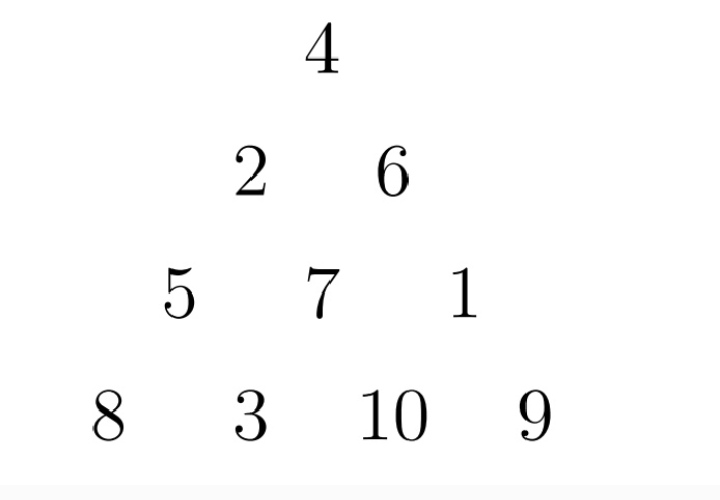
\includegraphics[width=\columnwidth]
		{./paid.jpg}
		\label{fig:fig1:0}
		\caption{function}
	\end{figure}
	Does there exist an anti-Pascal triangle with $2018$ rows which contains every integer from \begin{align}1 to 1+2 +....+2018?\end{align}
\item $A$ site is any point $(x,y)$ in the plane such that $z$ and $y$ are both positive integers less than or equal to $20$.Initially, each of the $400$ sites is unoccupied. Amy and Ben take turns placing stones with Amy going first. On her turn, Amy places a new red stone on an unoccupied site such that the distance between any two sites occupied by red stones is not equal to $sqrt(5)$ On his turn, Ben places a new blue stone on any unoccupied site. (A site occupied by a blue stone is allowed to be at any distance from any other occupied site.) They stop as soon as a player cannot place a stone. Find the greatest $K$ such that Amy can ensure that she places at least $K$ red stones, no matter how Ben places his blue stones
\item Let $a1,a2$,... be an infinite sequence of positive integers. Suppose that there is an integer $N\>1$ such that, for each $n\neq N$, the number $01$ is an integer. Prove that there is a positive integer $M$ such that for all $m1>=M$
\item $A$ convex quadrilateral $ABCD$ satisfies \begin{align}AB.CD=BC.DA.\end{align} Point $X$ lies inside. $ABCD$ so that \begin{align}\angle XAB=\angle XCD and \angle XBC=\angle XDA.\end{align} Prove that\begin{align}\angle BXA+\angle DXC=180^\circ\end{align}

\end{enumerate}
\end{document}
